\documentclass[11pt]{article}
\usepackage[T1]{fontenc}
\usepackage{lmodern,microtype}
\usepackage[a4paper,margin=28mm]{geometry}
\usepackage{amsmath,amssymb,amsthm,mathtools,bm}
\usepackage{graphicx,booktabs,array,enumitem}
\usepackage[numbers,sort&compress]{natbib}
\usepackage[colorlinks=true,linkcolor=blue!50!black,citecolor=blue!50!black,urlcolor=blue!50!black]{hyperref}
\usepackage{xcolor}
\usepackage{caption}
\usepackage{xurl}
\setcounter{tocdepth}{1}
\hypersetup{pdftitle={Irreversible Representation Growth under Logarithmic Loss: Sharp Four-State Constants and Source-Mass Order},pdfauthor={Wenyu Huang}}
\graphicspath{{../figures/}}
\newtheorem{theorem}{Theorem}[section]
\newtheorem{lemma}[theorem]{Lemma}
\newtheorem{proposition}[theorem]{Proposition}
\newtheorem{corollary}[theorem]{Corollary}
\theoremstyle{remark}\newtheorem{remark}[theorem]{Remark}
\newcommand{\KL}{D_{\mathrm{KL}}}
\newcommand{\E}{\mathbb E}
\newcommand{\Prob}{\mathbb P}
\newcommand{\cP}{\mathcal P}
\newcommand{\cH}{\mathcal H}
\newcommand{\Ropt}{R^*}
\DeclareMathOperator{\He}{He}
\title{Irreversible Representation Growth under Logarithmic Loss\\[4pt]
\large Sharp Four-State Constants and Source-Mass Order}
\author{Wenyu Huang\\University of California San Diego}
\date{}

\begin{document}
\maketitle
\begin{abstract}
Can increasingly informative representations be obtained by refining their
existing structure while remaining competitive at every capacity? We study
this question through the best prediction loss attainable with a bounded
number of representation states. A full-support family with four source
states and a binary target has minimum simultaneous log-loss ratio
$\sqrt{L}/(2\sqrt{\log 2})(1+o(1))$ over all deterministic hierarchies,
where the least source probability is $e^{-L}$. Allowing arbitrary stochastic
Markov refinements improves the sharp constant by a factor of two, but the
ratio remains unbounded. The conclusions concern total Bayes logarithmic
loss, hold with complete knowledge of the distribution, and use the smallest
possible nontrivial source and target cardinalities. We prove the deterministic
formula by enumerating all partitions and obtain the stochastic converse
through a finite random-function representation. A universal bound
$2+2\sqrt{3+\log(1/\gamma)}$ for four-state sources with masses at least
$\gamma$ proves that the worst-case order is
$\Theta(\sqrt{\log(1/\gamma)})$, for both deterministic and stochastic
refinements. Its proof uses a one-sided entropy perturbation bound to
control regrouping. We also give an excess-loss extension for convex
generators with divergent endpoint slope. The qualitative four-point
merge conflict is known; the contribution is its sharp, unbounded
all-hierarchy and stochastic quantification, together with explicit
regularity and reassignment boundaries. Reproducible high-precision
calculations evaluate every deterministic hierarchy and bracket the
stochastic optimum.
\end{abstract}
\tableofcontents

\section{Motivation and contribution}
Information can describe what a representation preserves without determining
whether a sequence of structural changes can realize the best representation
at each capacity. A system that only divides existing states has a particular
constraint: every later state must belong to one earlier state. Even an
oracle that knows the full task distribution cannot reverse an incompatible
earlier grouping through division alone. This distinction suggests studying
the \emph{price of irreversible growth}, rather than postulating that high
activation entropy should trigger neuron splitting.

We make the question precise for finite representations of a source $X$
used to predict a target $Y$. A representation with at most $k$ states incurs
Bayes logarithmic loss $H(Y\mid Z)$. The flat optimum $R_k^*$ can redesign
its encoder independently for every $k$. An irreversible growth path must
instead make its representations compatible: the coarser representation is
a function, or a stochastic degradation, of the finer one. This is an
abstraction of changes in representational organization. It does not
identify a representation state with a biological neuron, impose a specific
neural parameterization, or analyze gradient descent.

The principal result is stronger than the familiar observation that
capacity-specific optima need not be nested. For an explicit four-state
family, \emph{every} deterministic hierarchy has an arbitrarily large
multiplicative loss at either two or three states. Optimally chosen stochastic
encoders and stochastic coarsening do not remove this obstruction. Their
optimal asymptotic price is exactly half the deterministic price. These are
population statements about the admissible representations, with no
restriction on computation, sample size, or the information available to the
structural controller.

The constructive mechanism involves two common nearly deterministic inputs
and two rare intermediate inputs. At two states, the rare inputs join their
respective nearby anchors. At three states, the optimal representation
separates the anchors and groups the rare inputs together. The input weights,
posterior probabilities, and noise scale are chosen so that \emph{both}
possible ways to preserve a hierarchy become arbitrarily expensive relative
to the appropriate flat optimum. Irreducible label noise is smaller than the
relevant optimal risks, so the result applies to total prediction loss.

The dependence on rare source states admits a matching order theorem.
A universal square-root-logarithmic upper bound in the minimum source
mass holds for every four-state problem, without a lower bound on label
probabilities. A one-sided square-root entropy perturbation controls the
cost of moving the lighter member of an incompatible minimum-cost pair.
Balancing this hierarchy against a refinement of the optimal two-cell
partition proves the sharp source-mass order. Permitting reassignment of
one rare input, of mass $e^{-L}$, connects the two exact optima. A general
convex-generator theorem extends the excess-loss obstruction beyond Shannon
entropy. We give full proofs, including the elementary comparison inequalities
used in the positive result.

\section{Closest prior work and the novelty boundary}
Agglomerative information bottleneck (AIB) already optimizes task information
under hard partition cardinality and chooses merges by their information loss
\cite{slonim1999}. The extended report explicitly discusses the failure of
optimal partitions to form a hierarchy \cite[Section 3.1]{slonimreport}.
The objective and that qualitative observation are therefore established
starting points, not contributions of this manuscript.

The closest concrete precursor is Kartowsky and Tal
\cite[Section III-A, Example 1]{kartowsky2019}. Their binary-input,
four-output channel corresponds, after reversing the probabilistic roles,
to four equally weighted posterior points $0,1/3,2/3,1$. A middle-pair
merge conflicts with the best subsequent two-cell partition. Their main
result gives an additive worst-case power law for greedy degradation as the
output budget grows. Our question instead compares \emph{every} compatible
path with the flat optimum on the \emph{same instance} at two fixed budgets.
The rare-mass construction proves an unbounded multiplicative ratio, extends
it to total log-loss with full support, and resolves its stochastic
asymptotic constant. The underlying four-point pattern itself is not new.

The simultaneous approximation criterion is the price-of-hierarchy criterion
from hierarchical clustering; see Arutyunova and R\"oglin
\cite[Introduction and Section 2]{arutyunova2022,arutyunova2025}. Their sharp results
concern radius and diameter in metric spaces. KL centroid clustering belongs
to the established Bregman framework \cite[Sections 2--3]{banerjee2005}.
Chaudhuri and McGregor \cite[Theorem 8 and Lemmas 12 and 18]{chaudhuri2008}
compare KL clustering with Hellinger geometry and obtain logarithmic
approximation bounds for flat clustering. Their comparisons provide
background for our source-mass argument. A direct two-sided comparison
loses a logarithmic factor; the one-sided regrouping argument below instead
yields a square-root-logarithmic worst-case hierarchy bound. All analytic
inequalities used for this improvement are proved explicitly. Pointwise
functional domination is an established divergence-comparison method
\cite[Sections III-A and IV-B]{sason2016}; our scalar inequality is an
analytic tool for the regrouping bound, not a claim of a new comparison
principle.

Charvin, Catenacci Volpi, and Polani
\cite[Definition 5, Proposition 4, and Sections 2.3 and 3.2]{charvin2023} study exact and soft
successive refinement of the stochastic information bottleneck under
information-rate constraints. Their compatibility conditions and examples
make nonnesting a known issue in that setting as well. A rate constraint
$I(X;Z)\le R$ and a cardinality constraint $|\mathcal Z|\le k$ are
different resources. Our result uses the latter and quantifies the best
possible simultaneous multiplicative loss under hard alphabet budgets,
a different resource from their mutual-information tradeoff.

No \cite[Sections 2--3, Theorem 2]{no2019} proves successive refinability
for discrete memoryless source coding when the first decoder uses logarithmic
loss and the second uses an arbitrary distortion. That result concerns
asymptotic coding rates and reconstruction of the observed source. Here a
single-letter encoder observes $X$, predicts a separate noisy target $Y$,
and obeys fixed two- and three-state budgets. A guarantee under coding-rate
constraints does not imply a guarantee under these hard alphabet budgets.

The contribution considered here is the exact rare-mass theorem and its
stochastic coefficient, together with a matching worst-case source-mass
order proved by an explicit regrouping argument.
The standard loss identity, the nonnesting phenomenon, and the simultaneous
hierarchy criterion serve as established prerequisites.

\section{Statistical setting and admissible structural changes}
Let $X$ have a finite alphabet $\mathcal X$, positive masses $p_x$, and a
finite target alphabet $\mathcal Y$. Write $P_x=P(Y=\cdot\mid X=x)$.
All logarithms are natural, $0\log0=0$, and all entropies are finite.
A deterministic representation is a partition $\cP$ of $\mathcal X$;
its output identifies the cell containing $X$. For a cell $C$, put
\[
 p_C=\sum_{x\in C}p_x,\qquad
 P_C=p_C^{-1}\sum_{x\in C}p_xP_x.
\]
Predicting $P_C$ minimizes expected logarithmic loss conditional on $C$:
for any prediction $q$, its conditional expected loss equals
$H(P_C)+\KL(P_C\Vert q)$. Thus
\begin{align}
 R(\cP)&=H(Y\mid\cP(X))=\sum_C p_C H(P_C),\label{eq:risk}\\
 D(\cP)&=R(\cP)-B_0
   =\sum_C\sum_{x\in C}p_x\KL(P_x\Vert P_C),
 \quad B_0=H(Y\mid X).\label{eq:distortion}
\end{align}
The second identity follows by expanding the logarithms and using the
cell-mean formula. It also gives
$D(\cP)=I(X;Y)-I(\cP(X);Y)$. Hence minimizing total or excess
log-loss selects the same flat partitions, but their approximation ratios
are different when $B_0>0$.

Let $R_k^*$ and $D_k^*$ be the minimum risks over partitions into $k$
nonempty cells, for $1\le k\le |\mathcal X|$. Allowing at most $k$
cells gives the same value, since splitting a cell cannot increase
conditional entropy. A deterministic hierarchy $(\cH_k)_{k=1}^n$
has exactly $k$ cells at level $k$ and $\cH_{k+1}$ refines $\cH_k$.
Each step is a binary split in the growth direction. For $n=4$ define
\begin{equation}
 \rho_{\rm det}
 =\min_{\cH}\max_{k\in\{2,3\}}\frac{R(\cH_k)}{R_k^*}.
 \label{eq:det-price}
\end{equation}
Our full-support examples have positive denominators. Levels one and four
have fixed representations and ratio one, so omitting them changes nothing.

A stochastic refinement consists of channels $K_3:X\to Z_3$ and
$G:Z_3\to Z_2$, with at most three and two output states respectively.
The joint law is
\begin{equation}
 p(x,y,z_3,z_2)=p(x,y)K_3(z_3\mid x)G(z_2\mid z_3),
 \label{eq:markov}
\end{equation}
so $Y-X-Z_3-Z_2$ is a Markov chain. Define
\begin{equation}
 \rho_{\rm stoch}
 =\inf_{K_3,G}\max\left\{
 \frac{H(Y\mid Z_2)}{R_2^*},
 \frac{H(Y\mid Z_3)}{R_3^*}\right\}.
 \label{eq:stoch-price}
\end{equation}
This includes all deterministic hierarchies. No external random variable is
provided to the predictor for free in \eqref{eq:stoch-price}.

\begin{lemma}[Flat stochastic encoders do not improve the benchmark]
\label{lem:flat}
For finite $X,Y$ and a fixed output budget $k$, the minimum of
$H(Y\mid Z)$ over all channels $X\to Z$ with at most $k$ states is
$R_k^*$.
\end{lemma}
\begin{proof}
Every channel is a mixture of deterministic function tables: independently
sample the output assigned to each input according to its channel row.
Call the entire table $U$, independent of $(X,Y)$, and set $Z=f_U(X)$.
Its marginal channel is the desired one. Conditioning reduces entropy, so
$H(Y\mid Z)\ge H(Y\mid Z,U)=\E_U R(f_U)\ge R_k^*$.
A deterministic optimum attains equality in the minimum. If a function uses
fewer than $k$ cells, refine it to $k$ cells without increasing risk.
\end{proof}

\section{A sharp four-state obstruction}
For $L$ sufficiently large, set
\begin{equation}
 w=e^{-L},\qquad \varepsilon=w^2,\qquad
 \delta=\sqrt{\frac{\log2}{L}},\qquad c=\frac{1-2w}{2}.
 \label{eq:parameters}
\end{equation}
The source and binary-label posteriors are
\begin{center}
\begin{tabular}{lcccc}\toprule
Input & $A$ & $C$ & $D$ & $B$\\\midrule
Probability & $c$ & $w$ & $w$ & $c$\\
$\Prob(Y=1\mid X)$ & $\varepsilon$ & $\delta$ & $1-\delta$ & $1-\varepsilon$\\\bottomrule
\end{tabular}
\end{center}
Every entry of the joint distribution is positive. Symmetry gives
$\Prob(Y=1)=1/2$. Let $\rho_{{\rm det},L}$ and
$\rho_{{\rm stoch},L}$ denote \eqref{eq:det-price} and
\eqref{eq:stoch-price} for this law.

\begin{theorem}[Sharp deterministic and stochastic growth prices]
\label{thm:main}
The family \eqref{eq:parameters} satisfies
\begin{equation}
 \rho_{{\rm det},L}\sim\frac{\sqrt L}{2\sqrt{\log2}},
 \qquad
 \rho_{{\rm stoch},L}\sim\frac{\sqrt L}{4\sqrt{\log2}}.
 \label{eq:main}
\end{equation}
For all sufficiently large $L$, the unique flat optimal partitions, up to
cell labels, are
\[
 \cP_2^*=\{AC,DB\},\qquad \cP_3^*=\{A,CD,B\}.
\]
The deterministic formula also holds when every total risk in
\eqref{eq:det-price} is replaced by excess risk $D$.
\end{theorem}

We prove the deterministic assertion first; Section~\ref{sec:stochastic}
proves the stochastic assertion. The theorem excludes a universal constant
simultaneous guarantee even for an oracle structural controller. It is not
a computational hardness theorem.

\begin{figure}[t]
\centering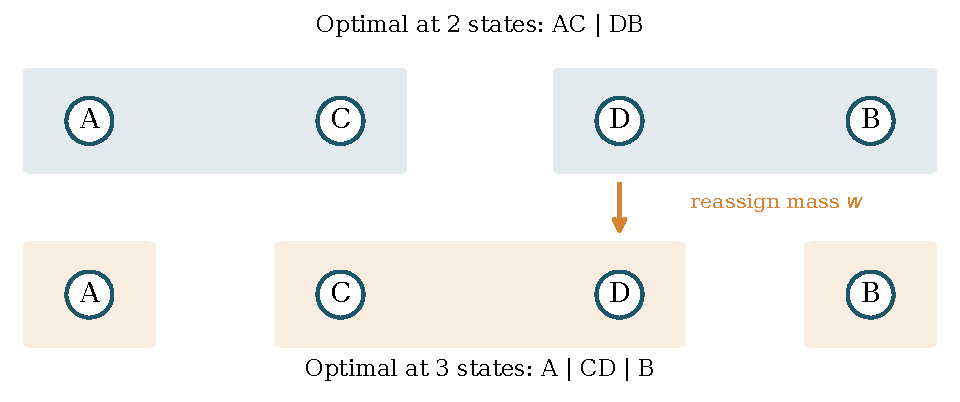
\includegraphics[width=.9\linewidth]{crossing_partitions_schematic.pdf}
\caption{Schematic of the incompatible flat optima. At two states the rare
inputs $C,D$ join their neighboring common anchors. At three states they
join each other. Splitting a cell of $\{AC,DB\}$ cannot produce
$\{A,CD,B\}$. Reassigning one rare input after a split can do so.
This illustration is schematic, not numerical evidence.}
\label{fig:schematic}
\end{figure}

\subsection{Exact reduction to six cluster costs}
Write $h(t)=-t\log t-(1-t)\log(1-t)$ and define
\[
 J(\alpha,\beta;s,t)
 =(\alpha+\beta)h\left(\frac{\alpha s+\beta t}{\alpha+\beta}\right)
       -\alpha h(s)-\beta h(t).
\]
This is the excess loss from merging two pure source states or two
already formed cells with masses $\alpha,\beta$ and posterior means $s,t$.
The cost of a triple is the cost of its first pair plus the cost of merging
that pair's mean with the third point; substitution in $J$ cancels the
intermediate entropy exactly. Define
\begin{align}
 a&=J(c,w;\varepsilon,\delta),&
 b&=J(c,w;\varepsilon,1-\delta),\nonumber\\
 r&=2w\{\log2-h(\delta)\},&
 q&=2c\{\log2-h(\varepsilon)\},\label{eq:six}\\
 t&=r+J(c,2w;\varepsilon,1/2),&
 u&=q+J(2c,w;1/2,\delta).\nonumber
\end{align}
Here $a$ is a near rare-anchor pair, $b$ a far pair, $r$ the rare pair,
$q$ the anchor pair, and $t,u$ are triples with one and two anchors.

\begin{lemma}[Complete partition enumeration]
\label{lem:enumeration}
The seven two-cell partition costs are $2a,2b,q+r,t,t,u,u$.
The six three-cell partition costs are $a,a,b,b,r,q$.
\end{lemma}
\begin{proof}
A two-cell partition has sizes $2+2$ or $1+3$. The three $2+2$ choices are
$AC|DB$, $AD|CB$, and $AB|CD$, with costs $2a,2b,q+r$.
The four $1+3$ choices isolate one of the two anchors (cost $t$) or one of
the rare inputs (cost $u$). A three-cell partition merges precisely one
pair; the six possible pairs have the listed costs. This covers every
partition, independently of posterior ordering or any clustering algorithm.
\end{proof}

\subsection{Asymptotic estimates with explicit noise scaling}
\begin{lemma}[The six costs and irreducible risk]
\label{lem:asymptotics}
Under \eqref{eq:parameters},
\begin{equation}
 a\sim w\delta L,\quad b\sim wL,\quad r\sim2w\log2,
 \quad t\sim wL,\quad q\to\log2,\quad u\to\log2,
 \label{eq:cost-asymptotics}
\end{equation}
and $B_0=2c h(w^2)+2w h(\delta)=o(w)$.
\end{lemma}
\begin{proof}
For $0<x\le1/2$ the Taylor expansion of $-\log(1-x)$, or its geometric
series integrated once, gives
\begin{equation}
 h(x)=x\log(1/x)+x+O(x^2),
 \label{eq:small-entropy}
\end{equation}
with an absolute remainder constant. We have $\delta\to0$,
$\delta L\to\infty$, and $\log(1/\delta)=O(\log L)=o(L)$.

Since $c+w=1/2$, the mean of the near pair is
$m=2w\delta+(1-2w)w^2$. On the interval between $2w\delta$ and $m$,
$h'(x)=\log((1-x)/x)=O(L)$. Thus
$h(m)=h(2w\delta)+O(w^2L)$. Using
$c h(w^2)=O(w^2L)$ and \eqref{eq:small-entropy},
\begin{align*}
 a&=w\delta\{L-\log(2\delta)+1\}-w h(\delta)+O(w^2L)\\
  &=w\delta(L-\log2)+O(w\delta^2+w^2L)
   \sim w\delta L.
\end{align*}
For the far pair, replace $\delta$ in the mean by $1-\delta$ and retain
$h(1-\delta)=h(\delta)$. This gives
\[
 b=w(1-\delta)\{L-\log(2(1-\delta))+1\}
        -w h(\delta)+O(w^2L)\sim wL.
\]
The formula for $r$ in \eqref{eq:six} gives its limit directly, as
$h(\delta)\to0$. The formula for $q$ gives $q\to\log2$.

The triple defining $t$ has mass $M=c+2w=(1+2w)/2$ and total positive-label
mass $z=cw^2+w=w+O(w^2)$. Equation~\eqref{eq:small-entropy} yields
\[
 M h(z/M)=z\{\log(M/z)+1\}+O(z^2/M)
         =w\{L-\log2+1\}+O(w^2L).
\]
Subtracting $c h(w^2)+2w h(\delta)$ proves
$t=wL+w\{1-\log2-2h(\delta)\}+O(w^2L)\sim wL$.

Finally $u\ge q$. Predicting $1/2$ after adding a rare state to the
anchor pair bounds its extra Jensen cost by
$w\KL(\operatorname{Ber}(\delta)\Vert\operatorname{Ber}(1/2))
\le w\log2$. Hence $u-q\in[0,w\log2]$ and $u\to\log2$.
The baseline statement follows because $h(w^2)=O(w^2L)$ and
$h(\delta)\to0$.
\end{proof}

The noise scale is substantive: $\varepsilon=w^2$ makes the baseline
$o(w)$. If one instead sets $w=\varepsilon^2$, a related excess-loss
example exists, but its baseline dominates the relevant distortion. Such
an example alone would not establish a total-risk ratio.

\subsection{The optimal deterministic hierarchy}
Define the total-risk ratios
\begin{equation}
 \alpha_L=\frac{B_0+a}{B_0+r},\qquad
 \beta_L=\frac{B_0+t}{B_0+2a}.
 \label{eq:alpha-beta}
\end{equation}
\begin{proposition}[Exact eventual formula and Pareto frontier]
\label{prop:pareto}
For all sufficiently large $L$, $D_2^*=2a$, $D_3^*=r$ and
\begin{equation}
 \rho_{{\rm det},L}=\min\{\alpha_L,\beta_L\}.
 \label{eq:exact-det}
\end{equation}
Every deterministic hierarchy's vector of total-risk ratios at levels two
and three is coordinatewise at least one of
$(1,\alpha_L)$ and $(\beta_L,1)$, and both vectors are attainable.
\end{proposition}
\begin{proof}
Lemma~\ref{lem:asymptotics} implies, eventually,
$b>a>r$, $q>a$, $t>2a$, and $t<q+r$, while $u$ and $q+r$ are bounded
away from zero. Thus the enumeration gives strict flat minima $2a$ and $r$.

If the three-cell partition merges $CD$, its possible two-cell costs are
$t,t,q+r$. Its best vector is $(\beta_L,1)$. If it merges a near pair,
such as $AC$, it can reach $AC|DB$ at level two and attains
$(1,\alpha_L)$. Any other three-cell merge has cost at least $a$, so its
level-three ratio is at least $\alpha_L$; its level-two ratio is at least
one by optimality of the benchmark. Both $\alpha_L$ and $\beta_L$ exceed
one eventually. These facts prove the Pareto statement and
\eqref{eq:exact-det}.
\end{proof}

As $B_0=o(w)$,
\[
 \alpha_L\sim\frac{\delta L}{2\log2},\qquad
 \beta_L\sim\frac1{2\delta}.
\]
Our choice of $\delta$ makes both asymptotic to
$\sqrt L/(2\sqrt{\log2})$. This proves the deterministic part of
Theorem~\ref{thm:main}. Setting $B_0=0$ in the ratio calculation proves
the excess-loss assertion. More generally, if $\delta\to0$ and
$\log(1/\delta)=o(L)$, the same estimates give
\[
 \rho_{{\rm det},L}=(1+o(1))
 \min\left\{\frac{\delta L}{2\log2},\frac1{2\delta}\right\}
\]
whenever $\delta L\to\infty$. Balancing these two terms explains the
selected family. The leading constants are sharp \emph{within that family};
Section~\ref{sec:sharp-source-mass} proves a matching worst-case order
over all four-state laws without identifying its sharp coefficient.

\section{Randomized hierarchies and stochastic refinements}
\label{sec:stochastic}
A random choice of a deterministic hierarchy is distinct from a stochastic
encoder used on each input. We first solve the former problem exactly and
then use it for a converse that covers the latter.

\begin{proposition}[Randomized hierarchy value]
\label{prop:randomized}
For sufficiently large $L$, the infimum over distributions on deterministic
hierarchies of
$\max_{k=2,3}\E R(\cH_k)/R_k^*$ equals
\begin{equation}
 \rho_{{\rm mix},L}
 =1+\frac{(\alpha_L-1)(\beta_L-1)}{\alpha_L+\beta_L-2}
 \sim\frac{\sqrt L}{4\sqrt{\log2}}.
 \label{eq:mix}
\end{equation}
\end{proposition}
\begin{proof}
Proposition~\ref{prop:pareto} permits replacing each hierarchy by one of
the two attainable Pareto vectors without increasing either expected
coordinate. Put probability $\lambda$ on $(1,\alpha_L)$ and
$1-\lambda$ on $(\beta_L,1)$. The coordinates are
$1+(1-\lambda)(\beta_L-1)$ and $1+\lambda(\alpha_L-1)$.
Their maximum is minimized at equality,
$\lambda=(\beta_L-1)/(\alpha_L+\beta_L-2)$, giving
\eqref{eq:mix}. The asymptotic follows from
$\alpha_L\sim\beta_L\sim\sqrt L/(2\sqrt{\log2})$.
\end{proof}

If instead the criterion is $\E\max_k R(\cH_k)/R_k^*$, randomizing
cannot improve the best deterministic value. Equation~\eqref{eq:mix}
uses the maximum of expected risks, which is the stronger lower-bound
setting needed next.

\begin{lemma}[Random-function converse for stochastic refinement]
\label{lem:stoch-lower}
Every pair of channels in \eqref{eq:markov} satisfies
\[
 \max_{k=2,3}\frac{H(Y\mid Z_k)}{R_k^*}\ge\rho_{{\rm mix},L}.
\]
\end{lemma}
\begin{proof}
Independently of $(X,Y)$, draw a table $F$ assigning a $Z_3$ value to
each $x$ according to $K_3(\cdot\mid x)$, with independent entries.
Draw a second table $G_0$ assigning a $Z_2$ value to each $z_3$ according
to $G(\cdot\mid z_3)$, also independently. The finite random variable
$U=(F,G_0)$ satisfies $Z_3=F(X)$ and $Z_2=G_0(F(X))$ and reproduces
the prescribed joint law. For each fixed $U$ these functions form nested
partitions with at most three and two cells.

These partitions can be refined to exactly three and two cells while
remaining nested and without increasing either risk. To see this, first
split fine cells until there are three. Each is still contained in an
original coarse cell. If there were two coarse cells, retain them; if
there was one, divide the three fine cells into two nonempty groups.
The resulting partitions extend to a complete four-state hierarchy by
adding the singleton and one-cell levels. Call this hierarchy $\cH^U$.
For each $k$, conditioning and refinement therefore give
\[
 H(Y\mid Z_k)\ge H(Y\mid Z_k,U)
   \ge\E_U R(\cH_k^U).
\]
Apply the definition of $\rho_{{\rm mix},L}$ to the distribution of
$\cH^U$. The random table is used only in a converse by revealing more
information; it is not assumed to be free information available to the
original encoder's predictor.
\end{proof}

\begin{proposition}[Matching stochastic construction]
\label{prop:stoch-upper}
A three-state encoder and deterministic two-state coarsening attain
\[
 \max_{k=2,3}\frac{H(Y\mid Z_k)}{R_k^*}
 \sim\frac{\sqrt L}{4\sqrt{\log2}}.
\]
\end{proposition}
\begin{proof}
For a fixed $\theta\in(0,1)$, use three outputs $0,m,1$ and the channel
\begin{center}
\begin{tabular}{c|ccc}
 & $0$ & $m$ & $1$\\\hline
$A$ & $1$ & $0$ & $0$\\
$C$ & $0$ & $1$ & $0$\\
$D$ & $0$ & $\theta$ & $1-\theta$\\
$B$ & $0$ & $0$ & $1$
\end{tabular}
\end{center}
Coarsen $0,m$ to one output and retain $1$ as the other. This directly
satisfies the output budgets; it does not use a public mixing label.

We calculate the leading entropies. The three-state middle output has mass
$w(1+\theta)$ and posterior
$[\delta+\theta(1-\delta)]/(1+\theta)$, so its risk contribution is
$O(w)$. Output $0$ contributes $c h(w^2)=O(w^2L)$. Output $1$ has mass
$c+(1-\theta)w\to1/2$ and failure-label mass
$c w^2+(1-\theta)w\delta\sim(1-\theta)w\delta$.
Equation~\eqref{eq:small-entropy}, together with
$\log(1/\delta)=o(L)$, shows that this contribution is
$(1+o(1))(1-\theta)w\delta L$. As $w=o(w\delta L)$,
\[
 H(Y\mid Z_3)\sim(1-\theta)w\delta L.
\]
At level two, the merged low output has mass
$c+w(1+\theta)\to1/2$ and positive-label mass
$c w^2+w\delta+\theta w(1-\delta)\sim\theta w$.
Its entropy contribution is $(1+o(1))\theta wL$; the other output
contributes only $O(w\delta L)$. Hence
$H(Y\mid Z_2)\sim\theta wL$.
By Lemma~\ref{lem:asymptotics}, $R_2^*\sim2w\delta L$ and
$R_3^*\sim2w\log2$. The two ratios are consequently asymptotic to
\[
 \theta\frac{\sqrt L}{2\sqrt{\log2}}
 \quad\text{and}\quad
 (1-\theta)\frac{\sqrt L}{2\sqrt{\log2}}.
\]
Choose $\theta=1/2$. Combining this feasible upper bound with
Lemma~\ref{lem:stoch-lower} and \eqref{eq:mix} proves both the proposition
and the stochastic part of Theorem~\ref{thm:main}.
\end{proof}

\section{Regularity, robustness, and the cost of reassignment}
\subsection{A sharp source-mass order for four-state sources}
\label{sec:sharp-source-mass}
The lower construction makes rare source states increasingly scarce. We now
show that its square-root-logarithmic order is the worst possible order for
four inputs. No lower bound on conditional label probabilities is needed.
The constants in the universal bound are not claimed to be optimal.

\begin{lemma}[A scalar logarithmic moment inequality]
\label{lem:log-moment}
Let $M\ge1$ and $0\le z\le M$. With continuous conventions at zero,
\[
 z(\log z)^2\le(2+\log M)(z\log z-z+1).
\]
\end{lemma}
\begin{proof}
For $0<z\le1$, put $t=-\log z\ge0$. The stronger inequality with
coefficient two is equivalent to
$t^2\le2(e^t-1-t)$, which follows from the exponential series.
For $z\ge1$, put $t=\log z\ge0$. The inequality with coefficient $2+t$
is equivalent to
\[
 t-2+(t+2)e^{-t}\ge0.
\]
The left side is zero at zero and has derivative
$1-(t+1)e^{-t}\ge0$. Since $t\le\log M$, the result follows.
Continuity handles $z=0$.
\end{proof}

\begin{lemma}[Square-root entropy perturbation]
\label{lem:entropy-lipschitz}
Let $\mu=(\mu_1,\ldots,\mu_m)$ be a positive probability vector. For
$u\in[0,\infty)^m$, define
\[
 E_\mu u^2=\sum_i\mu_i u_i^2,\qquad
 \operatorname{Ent}_\mu(u^2)
 =\sum_i\mu_i u_i^2\log\frac{u_i^2}{E_\mu u^2},\qquad
 F_\mu(u)=\sqrt{\operatorname{Ent}_\mu(u^2)},
\]
where $F_\mu(0)=0$. Then, for all nonnegative $u,v$,
\begin{equation}
 |F_\mu(u)-F_\mu(v)|
 \le\sqrt{2+\log(1/\min_i\mu_i)}
       \left(\sum_i\mu_i(u_i-v_i)^2\right)^{1/2}.
 \label{eq:entropy-lipschitz}
\end{equation}
\end{lemma}
\begin{proof}
First take strictly positive $u$ with $F_\mu(u)>0$. Put
$q=E_\mu u^2$ and $z_i=u_i^2/q$. Then
$z_i\le1/\mu_i\le1/\min_j\mu_j$, and differentiation gives
\[
 \partial_iF_\mu(u)=\frac{\mu_i u_i\log z_i}{F_\mu(u)}.
\]
Writing $C_\mu=2+\log(1/\min_i\mu_i)$, the squared gradient norm dual
to the weighted Euclidean norm satisfies
\begin{align*}
 \sum_i\frac{(\partial_iF_\mu(u))^2}{\mu_i}
 &=\frac{q\sum_i\mu_i z_i(\log z_i)^2}
          {\operatorname{Ent}_\mu(u^2)}\\
 &\le\frac{q C_\mu\sum_i\mu_i(z_i\log z_i-z_i+1)}
          {\operatorname{Ent}_\mu(u^2)}=C_\mu,
\end{align*}
where Lemma~\ref{lem:log-moment} and $\sum_i\mu_i z_i=1$ give the
last two steps. Cauchy--Schwarz bounds the derivative along a line segment
by $\sqrt{C_\mu}$ times its weighted speed.

For strictly positive $u,v$, the segment joining them has zero entropy
exactly at constant vectors. It either lies entirely in the line of constant
vectors, where the claim is immediate, or intersects that line at at most
one point. Integrate the derivative bound on the remaining intervals and
use continuity at their endpoints. For general nonnegative $u,v$, apply the
result to $u+\epsilon\boldsymbol{1},v+\epsilon\boldsymbol{1}$ and send
$\epsilon\downarrow0$. Their difference is unchanged and $F_\mu$ is
continuous, including at zero.
\end{proof}

The lemma is an analytic tool; the result below uses its one-sided effect
on a regrouping operation. It avoids paying a logarithmic comparison
factor on the distortion already incurred by the old partition.

\begin{theorem}[Four-state source-mass bound]
\label{thm:mass-bound}
If $|\mathcal X|=4$ and $p_x\ge\gamma>0$, there is a deterministic
hierarchy satisfying, simultaneously for $k=2,3$,
\begin{equation}
 D(\cH_k)\le K_\gamma D_k^*,\qquad
 R(\cH_k)\le K_\gamma R_k^*,\qquad
 K_\gamma=2+2\sqrt{3+\log(1/\gamma)}.
 \label{eq:mass-bound}
\end{equation}
The inequalities include zero-optimum cases without division.
\end{theorem}
\begin{proof}
Put $A=D_2^*$, $r=D_3^*$, and $C_\gamma=2+\log(1/\gamma)$.
Let $\cP_2$ be an optimal two-cell partition, and let $\{i,j\}$ be a
pair of minimum merge cost $r$. If $i,j$ belong to the same cell of
$\cP_2$, the partition merging only this pair refines $\cP_2$, so both
flat optima are simultaneously attained.

Otherwise let $a=p_i\le p_j=b$, exchanging their names if necessary.
Let $S,T$ be the cells of $\cP_2$ containing $i,j$, respectively, and
write $A_S=D(S)$, $A_T=D(T)$; thus $A=A_S+A_T$.
We move $i$ into $T$. In the new cell $T\cup\{i\}$, normalized source
weights are at least $\gamma$, since its total mass is at most one.
For each label $y$, apply Lemma~\ref{lem:entropy-lipschitz} to the vector
$(\sqrt{P_x(y)})_{x\in T\cup\{i\}}$ and to the vector with its
$i$th coordinate replaced by $\sqrt{P_j(y)}$. Multiply each resulting
square-root inequality by the square root of the cell mass, then use the
Euclidean triangle inequality across label coordinates to obtain
\begin{equation}
 \sqrt{D(T\cup\{i\})}
 \le\sqrt{D_{\rm rep}}+
      \sqrt{C_\gamma a\,\He^2(P_i,P_j)},
 \label{eq:one-sided-perturbation}
\end{equation}
where $D_{\rm rep}$ is the distortion of the artificial cell in which
$P_i$ is replaced by $P_j$, and
$\He^2(P,Q)=\sum_y(\sqrt{P(y)}-\sqrt{Q(y)})^2$.
The entropy expression equals KL cluster distortion by expanding each
label coordinate, so no probabilistic encoding claim is made about the
artificial replacement.

To bound $D_{\rm rep}$, evaluate its KL objective at the original centroid
$P_T$. The posterior $P_j$ now has weight $a+b\le2b$; every other
weight is unchanged. Minimizing over centroids can only help. Therefore
$D_{\rm rep}\le2A_T$.
Also $\KL(P\Vert Q)\ge\He^2(P,Q)$: writing
$f(z)=z\log z-z+1$, the scalar difference
\[
 f(z)-(\sqrt z-1)^2
 =2\sqrt z\{\sqrt z\log\sqrt z-\sqrt z+1\}\ge0
\]
proves this after multiplication by $Q$ and summation. The mixture
centroid of a positive-weight pair contains its members' supports.
The unconstrained weighted Euclidean centroid then gives
\[
 r\ge\frac{ab}{a+b}\He^2(P_i,P_j),\qquad
 a\He^2(P_i,P_j)\le2r.
\]
Thus \eqref{eq:one-sided-perturbation} implies
\[
 D(T\cup\{i\})\le
    \left(\sqrt{2A_T}+\sqrt{2C_\gamma r}\right)^2.
\]
Removing $i$ from $S$ cannot increase its distortion, by the Jensen
aggregation identity. The total new distortion $t$ is consequently bounded by
\begin{align}
 t&\le A_S+
        \left(\sqrt{2A_T}+\sqrt{2C_\gamma r}\right)^2\nonumber\\
  &\le\left(\sqrt{2A}+\sqrt{2C_\gamma r}\right)^2
   \le4A+4C_\gamma r.
 \label{eq:regrouping-bound}
\end{align}
For the second inequality use $A_S+2A_T\le2A$ and $A_T\le A$.
The moved cells are unions of the three fine cells
$\{i,j\},\{\ell\},\{m\}$. If removing $i$ empties $S$, split the
remaining cell into two nonempty unions of these fine cells. Refinement
does not increase distortion. This constructs a two-cell partition
compatible with the minimum-pair three-cell partition.

If $r=0$, the first bound in \eqref{eq:regrouping-bound} gives
$t\le2A$, and the fine distortion is zero; this also covers $A=0$.
Suppose $r>0$ and put $u=A/r\ge1$. Retaining $\cP_2$ and refining
it once yields fine distortion at most $A$, hence a simultaneous factor
at most $u$. The minimum-pair hierarchy constructed above has factor at
most $4+4C_\gamma/u$. Choose the better hierarchy. The increasing function
$u$ and decreasing function $4+4C_\gamma/u$ meet at
$2+2\sqrt{1+C_\gamma}$, so
\[
 \min\{u,4+4C_\gamma/u\}\le2+2\sqrt{1+C_\gamma}=K_\gamma.
\]
This proves the excess-loss claim. Adding the common nonnegative baseline
$B_0$ preserves any multiplicative factor at least one, proving the
statement for total risk.
\end{proof}

\begin{corollary}[Sharp worst-case source-mass order]
\label{cor:sharp-mass-order}
For $0<\gamma\le1/4$, take the supremum of $\rho_{\rm det}$, or
of $\rho_{\rm stoch}$, over four-state sources with masses at least
$\gamma$, arbitrary finite target alphabets, and positive flat total-risk
benchmarks. Both suprema have order
$\Theta(\sqrt{\log(1/\gamma)})$ as $\gamma\downarrow0$.
\end{corollary}
\begin{proof}
Theorem~\ref{thm:mass-bound} gives the upper bound; every deterministic
hierarchy is an admissible stochastic refinement. For the lower bound,
set $L=\log(1/\gamma)$ in Theorem~\ref{thm:main}. Its rare masses equal
$\gamma$ and its anchor masses exceed $\gamma$ eventually. Its positive
full-support total risks give the required lower order in both settings.
\end{proof}

The order is sharp over all four-state sources; the leading constants
in Theorem~\ref{thm:main} remain sharp only for the specified family.
The universal bound does not identify the extremal distribution or the
optimal worst-case coefficient. Rare source states are necessary for an
unbounded four-state price; extreme label probabilities alone do not suffice.


\subsection{Minimal cardinalities and perturbation robustness}
\begin{proposition}[Minimality and open-set robustness]
\label{prop:robust}
Four is the smallest source cardinality at which the deterministic
all-capacity hierarchy factor can exceed one. Two is the smallest
nontrivial target cardinality. For every finite $M$, a nonempty open set
of full-support four-by-two joint laws has both deterministic and
stochastic hierarchy price greater than $M$.
\end{proposition}
\begin{proof}
For at most three source states, only the two-cell level can be nontrivial;
any optimum there extends to the singleton and one-cell partitions. A
one-state target has zero prediction risk at every representation.
For robustness choose $L$ large enough that the mixed-hierarchy value in
\eqref{eq:mix} exceeds $2M$. There are finitely many deterministic
hierarchies. All their risk coordinates and positive flat benchmarks are
continuous functions of the full-support joint law. Their normalized
coordinate vectors therefore vary uniformly continuously locally. The
minimum over mixtures of the maximum of two expected coordinates changes
by at most the largest change in any coordinate. Thus it remains above
$M$ on some open neighborhood. The random-function converse applies to
every law on the same finite alphabets and bounds the stochastic and
deterministic prices below by this mixture value.
\end{proof}

\subsection{A vanishing amount of reassignment restores both flat optima}
Let $Z_2^*$ and $Z_3^*$ identify $\{AC,DB\}$ and $\{A,CD,B\}$.
A label-invariant measure of incompatibility is the minimum error in
recovering the old coarse label from the new fine label:
\begin{equation}
 \operatorname{rec}(Z_2^*\mid Z_3^*)
   =\min_g\Prob\{g(Z_3^*)\ne Z_2^*\}.
 \label{eq:recourse}
\end{equation}
\begin{proposition}[Exact reassignment cost]
\label{prop:recourse}
For the family \eqref{eq:parameters},
\[
 \operatorname{rec}(Z_2^*\mid Z_3^*)=w,
 \qquad H(Z_2^*\mid Z_3^*)=2w\log2.
\]
Splitting one cell and reassigning one input of mass $w$ connects the
optimal two- and three-cell partitions.
\end{proposition}
\begin{proof}
The singleton fine cells $A,B$ determine the old label exactly. In the fine
cell $CD$, of mass $2w$, the two old labels occur with equal conditional
probability. Any deterministic recovery map errs on at least one mass-$w$
input; assigning the cell to either old label attains that error. Its
conditional entropy is $\log2$, giving the entropy formula. To realize
the change, split $AC$ into $A$ and $C$, leaving $DB$ as the third cell;
then move $D$ from $DB$ into $C$. The result is $A|CD|B$ and the moved
source mass is exactly $w$.
\end{proof}

This is a statement about reassignment in the finite representation model.
It does not prescribe the parameter cost of moving a neuron's activation
region. It shows why measuring only state count or retained information
misses a separate resource: the ability to reorganize earlier assignments.

\section{An extension to convex Bayes-risk generators}
\label{sec:general-losses}

The logarithmic example has a broader counterpart for excess prediction
loss. This extension concerns the Jensen gap of a convex generator; it
does not assert the total-risk conclusion proved for logarithmic loss.
In particular, additive affine terms do not affect its distortion.

Let $\phi:[0,1]\to\mathbb R$ be continuous and strictly convex, and
differentiable on $(0,1)$. For a finite source with masses $p_x>0$ and
binary-label posteriors $\eta_x\in(0,1)$, define
\begin{equation}
 D_\phi(\mathcal P)
 =\sum_{C\in\mathcal P}\left\{
       \sum_{x\in C}p_x\phi(\eta_x)
       -p_C\phi(\bar\eta_C)\right\},
 \qquad
 p_C=\sum_{x\in C}p_x,\quad
 \bar\eta_C=p_C^{-1}\sum_{x\in C}p_x\eta_x.
 \label{eq:gen-distortion}
\end{equation}
This is the excess Bayes risk when the concave Bayes-risk function is
$-\phi$, up to an affine term, as in the convex representation of proper
scoring rules \cite[Theorem 1]{gneiting2007}. The identity follows by subtracting the
Bayes risk with the full source from that with the partition label.
Equivalently, putting
\begin{equation}
 d_\phi(z\Vert x)
 =\phi(z)-\phi(x)-\phi'(x)(z-x),
 \label{eq:gen-bregman}
\end{equation}
the distortion in \eqref{eq:gen-distortion} equals
$\sum_C\sum_{x\in C}p_xd_\phi(\eta_x\Vert\bar\eta_C)$, because the
linear terms sum to zero within every cell.

Write $D_{\phi,k}^*$ for the minimum of
\eqref{eq:gen-distortion} over partitions with $k$ nonempty cells.
For a four-state source, let
\begin{equation}
 \rho_\phi
 =\min_{\mathcal H}
   \max_{k\in\{2,3\}}
       \frac{D_\phi(\mathcal H_k)}{D_{\phi,k}^*},
 \label{eq:gen-price}
\end{equation}
where $\mathcal H$ ranges over complete binary-merger hierarchies.
The constructions below have four distinct posteriors, so both
denominators are strictly positive.

\begin{theorem}[Divergent endpoint slope]
\label{thm:gen-endpoint}
Suppose, in addition, that $\phi(x)=\phi(1-x)$ and
$\phi'(x)\to-\infty$ as $x\downarrow0$. Put
\[
 C=\phi(0)-\phi(1/2)>0,\qquad
 s_\varepsilon=-\phi'(\varepsilon),\qquad
 \delta_\varepsilon=\sqrt{C/s_\varepsilon}.
\]
There is a choice of positive $w_\varepsilon\le\varepsilon^2$ such
that the four-state source with masses
\[
 (p_A,p_C,p_D,p_B)=(c,w,w,c),\qquad c=(1-2w)/2,
\]
and posteriors
\[
 (\eta_A,\eta_C,\eta_D,\eta_B)
  =(\varepsilon,\delta,1-\delta,1-\varepsilon),
 \qquad w=w_\varepsilon,\quad\delta=\delta_\varepsilon,
\]
satisfies
\begin{equation}
 \rho_\phi
  \sim \frac{\sqrt{s_\varepsilon}}{2\sqrt C}
  \longrightarrow\infty
  \qquad(\varepsilon\downarrow0).
 \label{eq:gen-rate}
\end{equation}
All source and conditional label probabilities are positive for
sufficiently small $\varepsilon$.
\end{theorem}

\begin{proof}
We first justify a choice of $w$ that makes the required expansions
valid even when $\phi$ has no uniform second-derivative bound near
zero. For positive weights $\alpha,\beta$, define the weighted Jensen
gap
\[
 G(\alpha,\beta;x,z)
 =\alpha\phi(x)+\beta\phi(z)
  -(\alpha+\beta)\phi\left(
       \frac{\alpha x+\beta z}{\alpha+\beta}\right).
\]
If $m=(\alpha x+\beta z)/(\alpha+\beta)$, direct cancellation gives
\begin{equation}
 G(\alpha,\beta;x,z)
  =\beta d_\phi(z\Vert x)
       -(\alpha+\beta)d_\phi(m\Vert x).
 \label{eq:gen-small-weight}
\end{equation}
Fix an interior $\varepsilon$. Differentiability at $\varepsilon$
means
$d_\phi(\varepsilon+h\Vert\varepsilon)=o(|h|)$ as $h\to0$.
For $\alpha=c=(1-2w)/2$, $\beta=kw$, $k\in\{1,2\}$, and
$z\in[0,1]$, one has $|m-\varepsilon|\le4w$ for sufficiently
small $w$. Thus the remainder in \eqref{eq:gen-small-weight} is
$o(w)$ uniformly over these $k$ and $z$, with $\varepsilon$ fixed.
Since $s_\varepsilon\to\infty$, we may choose, separately for each
sufficiently small $\varepsilon$, a positive
$w=w_\varepsilon\le\varepsilon^2$ for which
\begin{equation}
 0\le
 kwd_\phi(z\Vert\varepsilon)
  -G(c,kw;\varepsilon,z)
 \le w/s_\varepsilon
 \quad
 (k\in\{1,2\},\ z\in[0,1]).
 \label{eq:gen-remainder-choice}
\end{equation}
The uniform statement follows directly from the definition of
differentiability on the shrinking interval
$[\varepsilon-4w,\varepsilon+4w]$; $w$ can be reduced further so
this interval is interior. This is an existence choice of the rare
mass, rather than an assumption of uniform differentiability as
$\varepsilon$ changes.

There are two useful preliminary limits. The supporting-line
inequality at $\varepsilon$ gives
\[
 0\le\varepsilon s_\varepsilon
 \le2\{\phi(\varepsilon/2)-\phi(\varepsilon)\}
 \longrightarrow0.
\]
It follows that $ws_\varepsilon\to0$ and
$\varepsilon/\delta\to0$, while
$\delta\to0$ and $\delta s_\varepsilon=\sqrt{Cs_\varepsilon}
\to\infty$. Strict convexity and symmetry imply $C>0$.

For clarity, write $s=s_\varepsilon$ and denote the six distinct
cluster costs by
\begin{align*}
 a&=G(c,w;\varepsilon,\delta),
 &b&=G(c,w;\varepsilon,1-\delta),\\
 r&=2w\{\phi(\delta)-\phi(1/2)\},
 &q&=2c\{\phi(\varepsilon)-\phi(1/2)\},\\
 t&=r+G(c,2w;\varepsilon,1/2),
 &u&=q+G(2c,w;1/2,\delta).
\end{align*}
Here $a,b$ are the near and far rare-anchor pair costs, $r,q$ are
the rare-pair and anchor-pair costs, and $t,u$ are the triple costs
with respectively one and two anchors. These expressions follow by
first merging the pair inside a triple and then merging its
centroid with the remaining point; expanding both sides proves
this aggregation identity exactly.

By \eqref{eq:gen-remainder-choice},
\[
 a=w\{\phi(\delta)-\phi(\varepsilon)
                  +s(\delta-\varepsilon)\}+o(w)
       \sim w\delta s,
 \qquad b\sim ws.
\]
The first equivalence uses boundedness of $\phi$ on $[0,1]$,
$\varepsilon s\to0$, and $\delta s\to\infty$; the second uses
the same bounds and $\delta\to0$. Continuity at the endpoints
gives $r\sim2wC$ and $q\to C$. Also,
\begin{align*}
 t
 &=2w\{\phi(\delta)-\phi(\varepsilon)\}
          +ws(1-2\varepsilon)+o(w)
   \sim ws.
\end{align*}
Finally, symmetry and differentiability imply $\phi'(1/2)=0$.
Applying \eqref{eq:gen-small-weight} at $1/2$ and using convexity
yields
\[
 0\le u-q\le wd_\phi(\delta\Vert1/2)
       =w\{\phi(\delta)-\phi(1/2)\}\le wC.
\]
Consequently $u\to C$.

We now check all possible partitions rather than assuming that a
particular merger algorithm is optimal. The seven two-cell costs
are $2a,2b,q+r,t,t,u,u$, and the six three-cell costs are
$a,a,b,b,r,q$. The limits just proved show that, for sufficiently
small $\varepsilon$,
\[
 D_{\phi,2}^*=2a,\qquad D_{\phi,3}^*=r.
\]
They also show $b>a>r$, $q>a$, $t>2a$, and $t<q+r$.
If a hierarchy merges the rare pair at level three, its possible
level-two costs are $t,t,q+r$, so its best factor is $t/(2a)$.
If it merges a near rare-anchor pair, it can attain the optimal
level-two partition and has best factor $a/r$. Every other
level-three pair has cost at least $a$, hence cannot improve on
the latter factor. We have therefore proved the exact eventual
formula
\[
 \rho_\phi=\min\{a/r,t/(2a)\}.
\]
Its two entries satisfy
\[
 \frac a r\sim\frac{\delta s}{2C}
            =\frac{\sqrt s}{2\sqrt C},
 \qquad
 \frac{t}{2a}\sim\frac1{2\delta}
            =\frac{\sqrt s}{2\sqrt C}.
\]
This proves \eqref{eq:gen-rate}.
\end{proof}

The choice of $w$ matters. For a general differentiable generator,
setting $w=\varepsilon^2$ without the further reduction in
\eqref{eq:gen-remainder-choice} need not justify the Taylor
remainder. The logarithmic constructions admit explicit estimates
and therefore do not require this adaptive choice. Moreover,
Theorem~\ref{thm:gen-endpoint} is a sufficient condition for an
unbounded hierarchy factor; it is not a characterization of all
generators with this property.

\begin{proposition}[A comparison on intervals of bounded curvature]
\label{prop:gen-curvature}
Let all posteriors lie in a fixed compact interval
$J\subset(0,1)$, and suppose $\phi$ is twice continuously
differentiable there with
$0<m\le\phi''(x)\le M<\infty$. Define weighted squared-error
distortion by
\[
 E(\mathcal P)=\sum_{C\in\mathcal P}
                  \sum_{x\in C}p_x(\eta_x-\bar\eta_C)^2.
\]
Then every partition satisfies
\begin{equation}
 \frac m2 E(\mathcal P)\le D_\phi(\mathcal P)
                         \le\frac M2 E(\mathcal P).
 \label{eq:gen-curvature-comparison}
\end{equation}
For any collection of cardinalities whose optimal distortions
are positive, the minimum simultaneous hierarchy factors obey
\[
 \frac mM\rho_E\le\rho_\phi\le\frac Mm\rho_E.
\]
\end{proposition}

\begin{proof}
The integral form of Taylor's theorem is
\[
 d_\phi(z\Vert x)
 =(z-x)^2\int_0^1(1-t)\phi''(x+t(z-x))\,dt.
\]
Both $x,z$ and their intervening segment belong to $J$, so this
expression lies between $m(z-x)^2/2$ and $M(z-x)^2/2$.
Summing at the cell centroids proves
\eqref{eq:gen-curvature-comparison}. Minimizing its two bounds
over all $k$-cell partitions gives the corresponding bounds on
optimal distortions. Dividing the partition bounds by these
optimal bounds, taking the maximum over cardinalities, and then
the minimum over hierarchies proves the last assertion.
\end{proof}

This comparison transfers hierarchy guarantees between the two
losses up to the fixed condition ratio $M/m$. It does not supply
an independent numerical constant for squared-error hierarchies.


\section{Reproducible computational investigations}
\label{sec:computations}
The experiments evaluate the mathematical objects directly. No neural
training run is needed to test a theorem about finite encoding channels,
and no empirical neural-network performance is inferred from these
calculations. An exploratory random search suggested the rare-anchor
pattern; its original script, seed, and rerun result are preserved separately.
The following calculations were specified after choosing the analytic family.

\subsection{Exhaustive evaluation and precision}
The program \texttt{code/quartet\_experiment.py} generates all fifteen set
partitions of four inputs, all seven two-cell partitions, all six
three-cell partitions, and all eighteen compatible three-to-two chains.
It evaluates their entropies with arbitrary precision, takes the exact
finite minimum numerically, and checks the formula in
Proposition~\ref{prop:pareto}. These are exhaustive finite comparisons,
not local optimization over selected starting points.

The scaling investigation uses fifteen values:
\[
 L\in\{16,24,32,48,64,96,128,192,256,384,512,768,1024,1536,2048\}.
\]
Decimal precision is $\lceil2L/\log10\rceil+90$, with a minimum of eighty,
so the small posterior $e^{-2L}$ is represented before subtracting
entropies. The parameters, baseline, partition costs, hierarchy scores,
and stochastic construction risks are saved as sixty-digit decimal strings.
Four representative cases,
including $L=2048$, are recalculated with seventy additional digits; the
saved deterministic prices, mixture values, stochastic bounds, and
construction risks agree to all sixty stored digits. Formula comparisons
use relative tolerance $10^{-40}$. This is numerical validation, not a
formal arithmetic certificate or a replacement for the proofs.

For random hierarchies, the program constructs the risk vectors of all
eighteen chains and checks the diagonal intersections of every pair of
vectors, as well as all vertices. The minimum of the maximum coordinate
on a convex polygon occurs at a vertex or a boundary intersection with
the diagonal, so this finite calculation recovers the mixture value. It
agrees with \eqref{eq:mix}. The explicitly specified stochastic encoder
with $\theta=1/2$ supplies an upper bound on $\rho_{\rm stoch}$; the
mixture value supplies a lower bound. We do not label the feasible
stochastic value as a finite-$L$ global optimum.

\begin{figure}[t]
\centering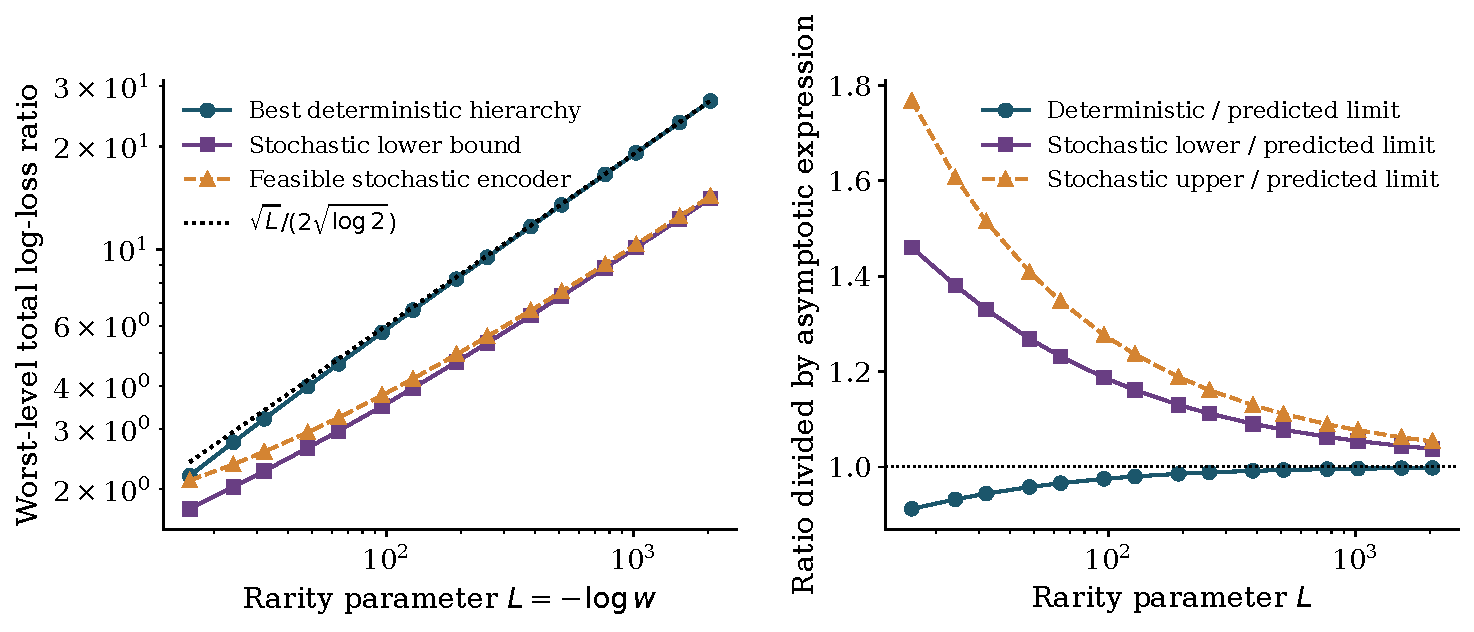
\includegraphics[width=\linewidth]{hierarchy_scaling.pdf}
\caption{Computed hierarchy prices and stochastic bounds from exhaustive
high-precision evaluation. Left: the best deterministic total-risk ratio,
the stochastic lower bound from random hierarchies, and the feasible
three-state stochastic encoder. Right: division by the respective predicted
asymptotic expressions; both stochastic bounds converge toward the same
constant. The stochastic upper curve is a feasible construction, not a
numerically certified global optimum.}
\label{fig:scaling}
\end{figure}

\subsection{Scale sensitivity and an unfavorable loss comparison}
At $L=256$ we vary
$\delta/\sqrt{\log(2)/L}\in\{0.35,0.5,0.65,0.8,1,1.2,1.5,2,2.5,3\}$.
The two competing excess-loss ratios move in opposite directions; their
minimum displays the predicted tradeoff. The finite-$L$ maximizing
multiplier need not equal the asymptotic choice one, since $h(\delta)$
corrections decay slowly.

The same distribution family is also evaluated under squared prediction
loss. Its excess Bayes risk is weighted posterior squared error. Every
sampled $L$ has an exactly compatible pair of flat optimal partitions and
computed hierarchy factor one. This control shows that the construction
is not a loss-independent impossibility; it reflects logarithmic loss's
sensitivity near the probability boundary. The bounded-curvature comparison
in Proposition~\ref{prop:gen-curvature} makes this distinction mathematical.

\begin{figure}[t]
\centering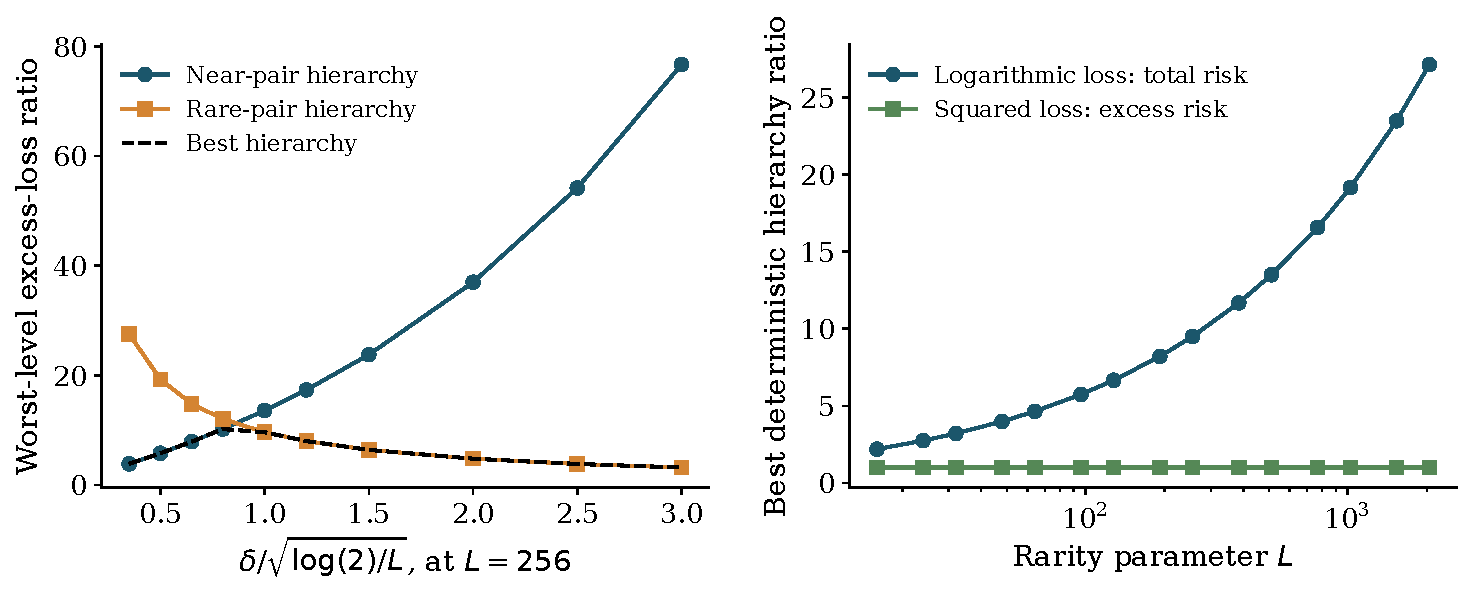
\includegraphics[width=\linewidth]{sensitivity_and_loss.pdf}
\caption{Computed sensitivity and loss comparison. Left: changing the
intermediate posterior scale at $L=256$ trades the cost of near-pair and
rare-pair hierarchies; the dashed line is the best excess-loss ratio.
Right: the same source family has growing total-log-loss hierarchy price,
while its squared-loss excess hierarchy price equals one on all evaluated
cases. The two curves use the explicitly indicated loss criteria.}
\label{fig:sensitivity}
\end{figure}

\begin{table}[ht]
\centering
\begin{tabular}{rrrrrr}
\toprule
$L$ & $\log_{10}w$ & $\rho_{\rm det}$ & Stochastic lower & Feasible upper & $B_0/D_3^*$\\
\midrule
16 & -6.9 & 2.19133 & 1.75386 & 2.12340 & 2.81549\\
64 & -27.8 & 4.64119 & 2.95855 & 3.23657 & 0.92962\\
256 & -111.2 & 9.49943 & 5.34252 & 5.57974 & 0.41840\\
1024 & -444.7 & 19.14974 & 10.13188 & 10.34765 & 0.21067\\
2048 & -889.4 & 27.12538 & 14.10659 & 14.31553 & 0.15253\\
\bottomrule
\end{tabular}
\caption{Selected computed values. The deterministic column uses total risk. The stochastic columns are a variational lower bound evaluated numerically and the risk of the explicit encoder, respectively. The underlying values are saved with sixty significant decimal digits.}
\label{tab:results}
\end{table}


The absolute losses approach zero as $L$ grows, while their ratios diverge.
This is a failure of a uniform multiplicative guarantee near a highly
predictable target, not a lower bound on fixed-scale absolute damage.
The source masses become extremely small: at $L=2048$, the rare mass is
about $10^{-889}$. Ordinary random sampling would not expose such states
at practical sample sizes. The computation uses a known finite population
law to make the theorem inspectable; it does not establish practical
learnability of the rare states.

\subsection{Numerical challenges to the source-mass proof}
The new bound is supported by executable mathematical checks, separate
from the deterministic family calculations. With seed 20260914,
\texttt{research/sharp\_rate\_check.py} generates 4,000 entropy vectors
in dimensions two through sixteen, including zero coordinates and constant
vectors, and 1,204 four-state distribution cases with target sizes two
through eight. Four distribution cases explicitly include identical
posteriors, a constant target, or duplicate pairs. Every distribution case
enumerates all partitions and compatible chains; fourteen cases are
recalculated at 90 decimal digits. Raw vectors and distributions are saved.

All executed checks satisfy the asserted bounds within the documented
floating-point tolerance. The largest computed squared Lipschitz ratio
relative to its bound is 0.92884; the largest gradient ratio is 0.93670.
These are adversarial diagnostics rather than proofs, samples from a
learning problem, or a search certificate for the worst-case constant.
Near-zero floating-point ratios are omitted from ratio summaries, and
explicit degeneracies remain in the high-precision checks.

\begin{figure}[t]
\centering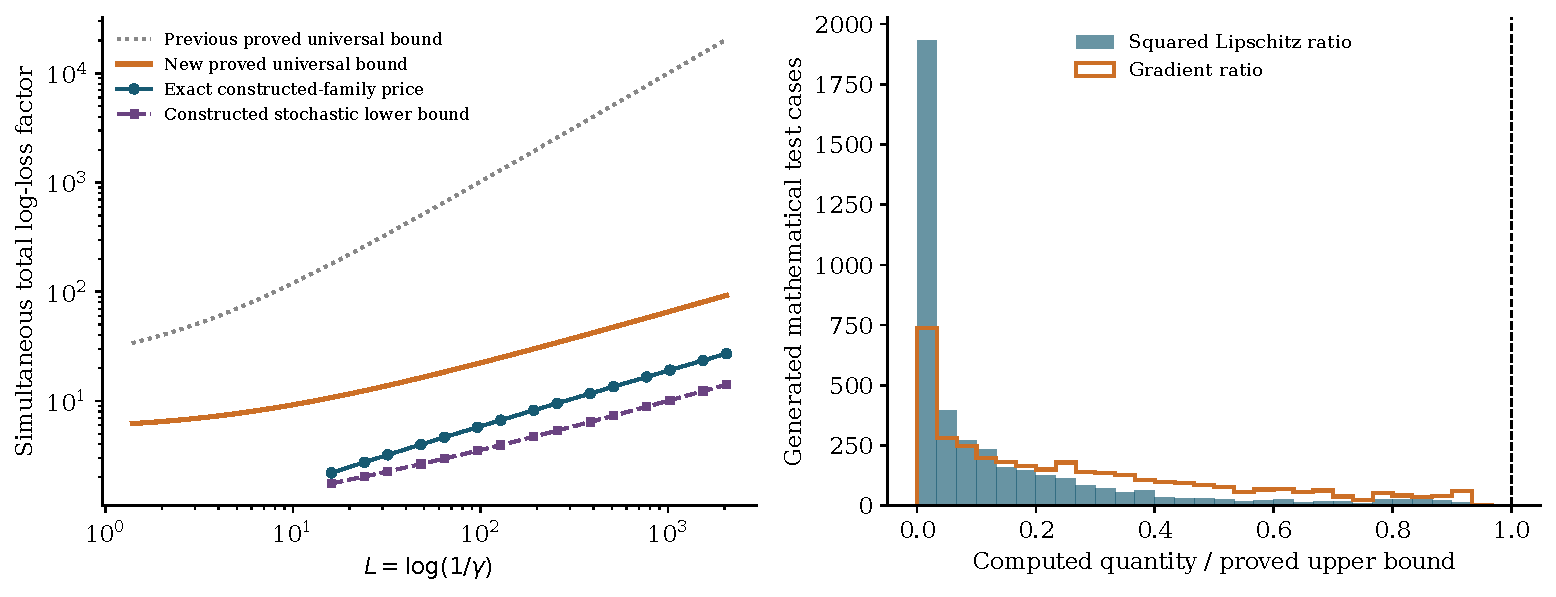
\includegraphics[width=\linewidth]{sharp_source_mass.pdf}
\caption{Left: the earlier logarithmic universal bound, the new proved
square-root-logarithmic envelope, and independently enumerated values for
the explicit family. The envelope is a theorem, not a numerical optimizer
output. The stochastic lower curve remains a lower bound rather than an
exact finite-parameter optimum. Right: distributions of the ratios tested
in 4,000 generated entropy-vector cases; one is the proved ceiling. These
mathematical checks do not replace the proofs.}
\label{fig:sharp-source-mass}
\end{figure}

\section{Interpretation and remaining questions}
Information-guided structural adaptation requires specifying \emph{which
structural operations information is allowed to guide}. In this finite model, the
controller can know the exact task distribution, evaluate every partition,
and use arbitrary computation. A restriction to nested refinements still
prevents a uniform approximation guarantee. The obstruction is therefore
not repaired by a more accurate entropy estimator or a more sophisticated
split score alone.

The conclusions also separate two resources often grouped under capacity.
A third state makes the independently optimal representation better, but
reaching it may require moving information across an old boundary.
Stochastic routing reduces the asymptotic price by exactly two in the
constructed family. Full reassignment of a mass-$w$ input restores both
flat optima. State count, stochasticity, and reassignment are distinct
resources in this analysis.

Several limitations delimit the result. The model counts discrete
representation states, not parameters, real-valued feature coordinates,
neurons, or energy. It permits Bayes-optimal decoding and assumes a known
joint law. It concerns the two specific intermediate budgets, so a process
that skips a budget is outside the simultaneous guarantee. It does not
exclude effective growth rules for restricted distributions, finite-sample
objectives, additive accuracy criteria, or architectures that naturally
reorganize representations. The full-support and open-neighborhood results
remove exact zeros and exact symmetry as requirements for a given finite
gap, but the size of that neighborhood need not be uniform in $L$.

The worst four-state source-mass order is
$\Theta(\sqrt{\log(1/\gamma)})$. The optimal worst-case leading
coefficient and extremal laws remain unknown. The endpoint-slope theorem gives a
sufficient condition for excess-loss obstruction, but no necessary and
sufficient classification of scoring rules. A broader research direction
is to characterize how a limited reassignment budget controls the price
of structural growth. These questions are not needed for the established
theorems and remain unresolved in this work.

\clearpage
\begingroup
\small\raggedright
\bibliographystyle{plainnat}
\bibliography{references}
\endgroup
\end{document}
